\subsection{Emergency Services Crew}
\begin{enumerate}

    \item \textbf{Receive and Assess Call.} 
    The \textit{Emergency Call Agent} receives incoming calls and collects relevant details about the incident. 
    This task requires human input for accurate interpretation and contextual understanding of the caller's description, 
    ensuring critical information is gathered effectively. The information that this agent receives answers the following 
    six questions and is saved in a report:
    \begin{itemize}
        \item What type of fire is it? E.g. ordinary, electrical, gas, etc.
        \item Where is it? The location is received as coordinates \((x, y)\).
        \item Is anyone injured? How badly? The answer will be a list of strings, detailing the risk level of each person. If the list 
        if empty then there will be no injured people and it will be unnecessary to report it to the \textit{Medical Service Crew.}
        \item How severe is the fire? It will be considered as low, medium or high.
        % extra inputs
        \item Are there hazards? Examples of hazards could include gas cylinders, chemicals, explosions, etc.
        \item Is it an indoor or outdoor fire? The answer will be either \textit{outdoor} or \textit{indoor}.
        \item Is anyone inside or trapped? The answer will be an integer number $M$ representing the number of trapped people. 
        If $M > 0$, rescues are needed, and the \textit{Notification Agent} will detail that to the Fire Fighters Crew.
    \end{itemize}
    

    \item \textbf{Notify Other Crews Decision.} 
    The \textit{Notification Agent} receives the details about the fire then it decides which crew should be notify and send
    all the information to the flow. It also decides whether the medical services are required or not, depending on the 
    human input related to the injured individuals.    

\end{enumerate}

\paragraph{Task Dependencies:}

The sequential workflow for the Emergency Services Crew depends on task dependencies to ensure efficiency and coordination:
\begin{itemize}
    \item The \textit{Notify Other Crews Task} depends on the completion of the \textit{Receive and Assess Call Task}, which 
    involves human input to accurately assess and interpret the situation.
\end{itemize}


The task dependencies and agents who perform each task can be observed in Figure~\ref{fig:emergency_services_flow}.

\begin{figure}[h!]
	\centering
	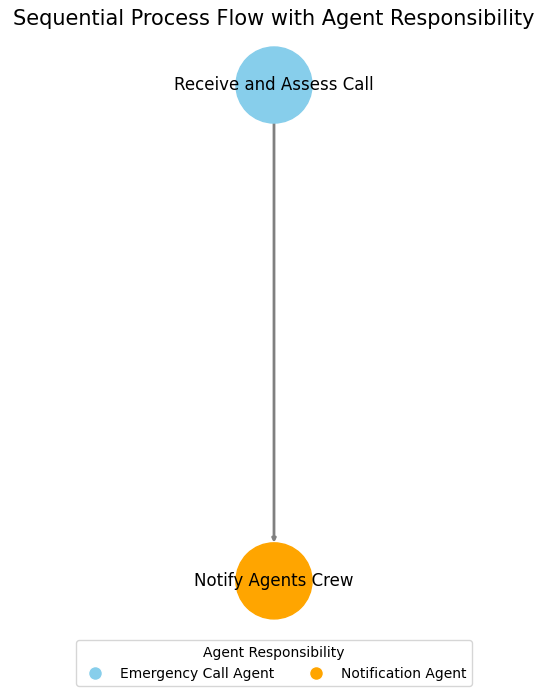
\includegraphics[height=0.4\textheight]{figures/emergency_services_crew_flow.png}
	\caption{Sequential Process Flow of the Medical Services Crew with Agent Responsibilities}
	\label{fig:emergency_services_flow}
\end{figure}
